\documentclass[12pt]{article}
\usepackage{graphicx}
\usepackage{amsmath}
\usepackage{hyperref}
\usepackage{caption}
\usepackage{float}
\usepackage{titlesec}

\usepackage[margin=1in]{geometry}
\titleformat{\section}{\normalfont\Large\bfseries}{\thesection}{1em}{}
\titleformat{\subsection}{\normalfont\large\bfseries}{\thesubsection}{1em}{}

\title{NOMAD Notes}
\author{Authors \ Mathematics and Computing \\ Indian Institute of Technology}
\date{\today}

\begin{document}
\maketitle
\section{Introduction}
\begin{quote}
In this paper, we present a design for such a policy by
combining a Transformer backbone for encoding the high-
dimensional stream of visual observations with diffusion
models for modeling a sequence of future actions and instan-
tiate it for the particular problem of visual exploration and
goal-seeking in novel environments
\end{quote}
\textbf{What is nomad?}\\
NoMaD is a robot navigation system that can:
\begin{itemize}
    \item Explore unknown places on its own (goal-agnostic behavior).
    \item Go to a specific place or object when given a goal image (goal-directed behavior).
\end{itemize}
The key idea: Instead of having two different systems for these tasks (like other methods do), NoMaD does both using one unified model.\\

\textbf{Why is this important?}\\

In the real world:\\
-A robot might need to search for a place (like exploring a building).\\
-Later, it may need to go back to that place (like retrieving an object from a room).\\
-Existing systems often split these into two steps — exploration and navigation — with different models or planning stages.\\
NoMaD combines both into one model, making the robot:\\
\ -Smarter.\\
\ -Faster.\\
\ -Less prone to mistakes (like collisions).\\

\textbf{How does it work?}\\

Input: An image of the environment, and optionally a goal image (like “go here”).\\
Model: Uses a Transformer (like those in NLP/AI) to understand the visual world, and a Diffusion Model to plan actions.\\
Goal Masking: If a goal image is given, it uses that to guide movement. If not, it goes into exploration mode.\\
This "masking" lets the model ignore the goal if it doesn't have one, which allows exploration to happen naturally.\\

\textbf{Why Diffusion Models?}\\
Diffusion models are great at generating complex, multi-modal outputs. That means:\\
The robot doesn’t just plan a single path.\\
It can consider many possibilities, which helps it handle real-world messiness (like obstacles or uncertainty).\\
\
We factorize the exploration problem into (i) learned control
policies that can take diverse, short-horizon actions, and (ii)
a high-level planner based on a topological graph that uses
the policy for long-horizon goal-seeking
\bigskip
\begin{quotation}
    Exploring a new environment is often framed as the problem of efficient mapping....
\end{quotation}
Robots exploring a new area are essentially trying to map it efficiently—this means covering as much area as possible, ideally without wasting time.\\
Some methods use local control strategies (e.g., make decisions based only on nearby information), and others use global strategies (like "frontier exploration", which targets unexplored boundaries).\\
However, making very accurate 3D maps is hard, especially if the robot doesn't have good depth sensors.\\
\begin{itemize}
    \item Some approaches use simulation data (training in virtual environments).
    \item  Others learn from real-world data directly.
    These models may use:\\
    \ Intrinsic rewards: Encouraging the robot to explore new things.\\
    \ Semantic prediction: Going to interesting or informative places.\\
    \ Latent variable models: Abstract models of how actions affect the world.
\end{itemize}

\textbf{Challenge!}\\
Even the best learning-based models trained in simulation don't transfer well to real-world environments, and many fail in complex spaces.\\

\textbf{Enter NoMaD: A New Method}\\
ViNT is a previous system that used a big model to suggest where the robot should go next by generating subgoal images.\\
NoMaD improves on this by:
\begin{itemize}
    \item Not generating images.
    \item Directly predicting actions using diffusion models, which are typically used in image generation tasks but can model complex probabilities really well.
    \item This makes NoMaD more accurate and much lighter (needs 15x fewer parameters).
    \item It’s so efficient, it can run on low-power devices like a Jetson Orin (a type of small computer often used in robots).
\end{itemize}
\bigskip
In exploration, there can be many possible good actions at any moment (multi-modal distribution)\\
Diffusion models are powerful because they can learn complex distributions (e.g., "what are all the good things I might do next?") without needing to simulate the future.\\
Nomad adds goal-conditioning to diffusion-based action generation, meaning it can do both:\\
-Goal-directed exploration (e.g., "go there")\\
-Undirected exploration (e.g., "explore as much as you can")\\
\section*{Goal: A Visual Navigation Policy}
The authors want to build a control policy (called $\pi$) that lets a robot navigate using only its camera (RGB images). The robot:
\begin{itemize}
    \item Takes in past and current camera images $(o_t := o_{t-P :t})$
    \item Outputs the distribution over future actions ($(a_t)$:=$a-{t:t+H}$)
    \item Might also be given an image of a goal ($o_g$) to help guide it.
\end{itemize}
There are two possible cases:
\begin{itemize}
    \item If a goal image is provided, $\pi$ tries to move the robot toward the goal.
    \item If no goal is given (like in exploration tasks), $\pi$ should still act safely (avoid obstacles, stay on paths) and explore effectively.
\end{itemize}
To manage longer-term planning, the robot also uses:
\begin{itemize}
    \item A topological Memory $\mathcal{M}$ (a kind of virtual memory map)
    \item A high-level planner to help decide where to explore next.
\end{itemize}
\subsection*{Visual Goal-Conditioned Policies (ViNT as Backbone)}
They use ViNT (Visual Navigation Transformer), which is based on the Transformer architecture (very popular in modern AI).\\
How ViNT works:
\begin{itemize}
    \item Each image (current or past) is passed through an EfficientNet-B0 encoder to extract features.
    \item The goal image and current state are combined via a special goal fusion encoder.
    \item The resulting features (called tokens) are fed through Transformer attention layers, producing a context vector $c_t$.
    \item This vector is then used to predict future actions ($a_t$) and temporal distance to the goal ($d(o_t, o_g)$).
\end{itemize}
These predictions are trained using supervised learning (the model is shown what the correct actions and distances should be and learns from that).\\
\begin{quote}
    But: ViNT only works if there is a goal image. It can't explore on its own
\end{quote}
To enable the robot to operate in large, complex environments, it needs more than just immediate camera inputs.\\
So, they introduce: A topological memory $\mathcal{M}$
\begin{itemize}
    \item A graph where each node is a past visual observation.
    \item Edges connect nodes that the robot can travel between, using ViNT's predicted distances to know which transitions are possible.
\end{itemize}
When a robot can’t reach a goal directly using visual input, it uses this graph $\mathcal{M}$ to plan a path via intermediate goals (subgoals).
Even without a specific goal, this graph helps the robot explore logically and not just randomly.\\
\subsection*{Frontier-Based Exploration}
In this work, they test NoMaD's ability to propose diverse subgoals and explore unseen areas using a frontier-based method:
\begin{itemize}
    \item Frontier = edge between explored and unexplored space.
    \item The robot is encouraged to go to frontiers, gradually covering new space.
\end{itemize}
They adopt the framework from ViKiNG, but replace the old policy with NoMaD, which can now do both:\\
Goal-seeking (when a goal is provided)\\
Exploration (when no goal is provided)\\
\section*{Methods}
\begin{figure}[H]
    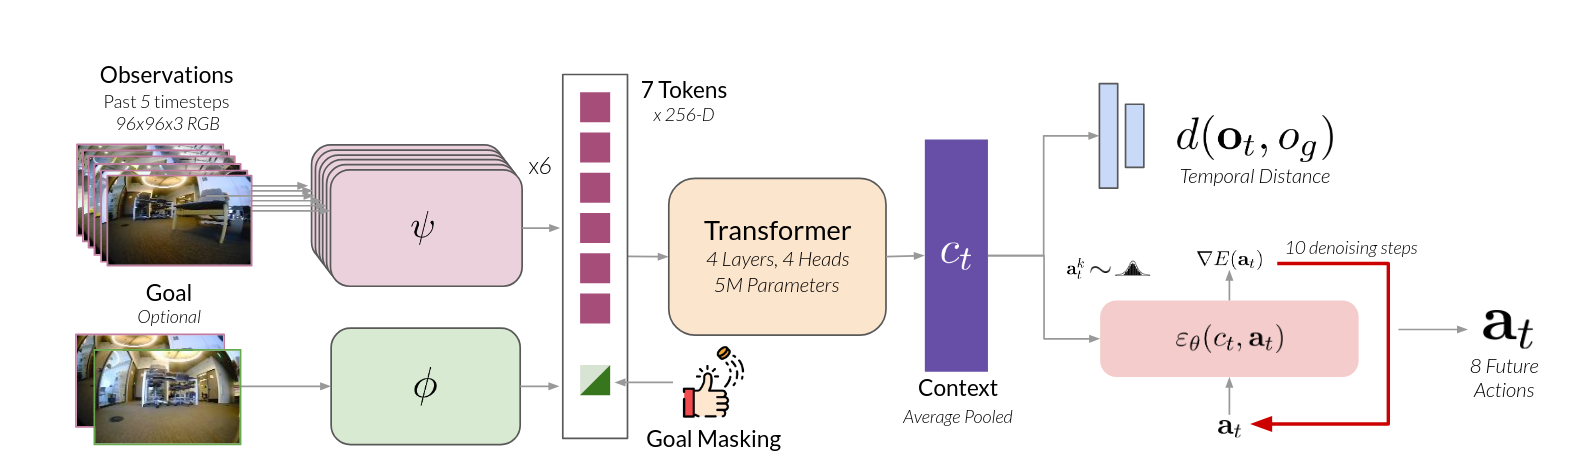
\includegraphics[width=1\textwidth]{nomad_diagram.png}
    \caption{Overview of the NoMaD architecture. The model takes in RGB images and outputs a distribution over future actions. It can also use a goal image to guide its actions.}
    \label{fig:nomad_diagram}
\end{figure}
\subsection*{A. Goal Masking}
The idea is based on the ViNT architecture, which uses Transformer layers to encode inputs.\\
New in NoMaD:\\
They introduce a binary variable m, the goal mask.\\
\begin{itemize}
    \item m=0: Goal is visible $\to$ conditioned on goal image.
    \item m=1: Goal is hidden $\to$ acts without knowing any goal.
\end{itemize}
\textbf{training}:\\
sample m ~ Bernoulli($p_m$) where $p_m$ = 0.5\\
-- 50 \% of the training time, goal provided.\\
-- 50 \% of the training time, no goal (exploratory behavior).\\
This balance allows shared weights to generalize across both behaviors.\\

\noindent \textbf{Modified Transformer Input:}\\
\[ c_t = f(\psi(o_i), \phi(o_t, o_g), m) \]
Where:\\
\begin{itemize}
    \item $c_t$ = context vector
    \item $\psi$ and $\phi$ = visual encoders
    \item $o_i$ = current image
    \item $o_t, o_g$ = time-step and goal image
    \item m = goal mask
    \item f = Transformer function (ViNT style)
\end{itemize}
Masking is applied in the attention layers, so goal embeddings are ignored if m=1.\\
\subsection*{B. Diffusion Model}
In general, diffusion models are generative models.
They work by gradually adding noise to data (a forward process), and then learning to remove that noise (a reverse denoising process) to generate realistic samples.

In NoMaD, instead of generating images or audio, the diffusion model is used to generate robot actions — specifically, the next velocity command (like linear and angular speed) that’s safe and goal-aligned.\\

Action spaces in navigation are multimodal. Need to avoid actions leading to collisions.\\
\textbf{diffusion model setup:}\\
They model the conditonal distrubution of the next action $a_t$ as\\
\begin{center}
    $p(a_t|c_t)$
\end{center}
Here's how it works:\\
\textbf{The Forward Diffusion Process (Add Noise)}\\
1. Start with a real action $a^{0}_t$  from the dataset.\\
Then we add gaussian noise over multiple steps k = 1 to K.\\
\begin{center}
    $a^{k}_t = \sqrt{\alpha_k} a^{k-1}_t + (\sqrt{1 - \alpha_k}) \epsilon$
\end{center}
where:\\
\begin{itemize}
    \item $\epsilon$ ~ $\mathcal{N}$(0,I) is a random noise
    \item $\alpha_k$ is a noise scheduler (eg square cosine )
    \item By step K, the action is almost pure noise.
\end{itemize}
This is only used during training.\\
\textbf{Reverse Denoising (Learned Model)}\\
2. The model learns how to reverse this process:\\
\begin{itemize}
    \item starting from pure noise $a^{k}_t$~$\mathcal{N}(0,I)$, it denoises step by step to recover the final clean action $a^{0}_t$.
    \item Each denoising step is:
    \[ 
    a^{k-1}_t = \alpha(\alpha^{k}_t-\gamma_k.\epsilon_{\theta}(c_t, a^{k}_t,k)) + \mathcal{N}(0,\sigma^2.I)
    \]
\end{itemize}
Where:
\begin{itemize}
    \item $\epsilon_{\theta}$ is a neural network (UNet) that predicts the noise.
    \item $c_t$ is the context vector from the Transformer.(images,goal mask)
    \item k: current diffusion step.
    \item $\gamma, \alpha ,\sigma$ are scheduler constants.
\end{itemize}
\textbf{What is the Network $\epsilon_{\theta}$ Like?}
It's a 1-D conditional UNet.\\
-- 15 convulational layers.\\
-- Takes in : the noisy action $a^{k}_t$, the context vector $c_t$, and the diffusion step k.\\
-- Outputs the predicted noise vector $\hat{\epsilon}_k$\\
During training, it is compared to the true noise added earlier.\\
\textbf{Training Objective}\\
The loss is just Mean Squared Error (MSE) betweeen the predicted and the actual noise. For overall loss function, we add the MSE temporal distance loss to the objective function.\\
\begin{center}
   \[ 
   \mathcal{L}_{NOMAD}(\phi,\psi,f,\theta,f_d) = MSE(\epsilon^{k}, \epsilon_{\theta}(c_t, a^{0}_t + \epsilon^{k},k)) + \lambda .MSE(d(o_t, o_g), f_{d}(c_t))
   \]
\end{center}
where:\\
\begin{itemize}
    \item $\psi$,$\phi$ correspond to the visual encoders for the observation and goal images.
    \item $f$ corresponds to the transformer layers,
    \item $\theta$ corresponds to diffusion process parameters,
    \item $f_d$ corresponds to the temporal distance predictor.
    \item $\lambda$ = 10^{-4} is a hyperparameter that controls the relative weight of the temporal distance loss
    \item $p_m$ = 0.5 is the goal mask probability.
    \item Square Cosine Noise Scheduler is used.
    \item The model is trained using AdamW optimizer with a learning rate of 1e-4.
    \item Model is trained for 30 epochs, with batch size of 256.
    \item We use cosine scheduling and warmup to stabilize the training process and follow other hyperparameters from ViNT 
    \item For the ViNT observation encoder, we use EfficientNet-B0 to tokenize observations and goals into 256-dimensional embeddings, followed by a Transformer decoder with 4 layers and 4 heads.
\end{itemize}

\end{document}